\documentclass{article}
\usepackage{amsmath}
\usepackage{amssymb}
\usepackage{enumitem}
\usepackage{graphicx}
\usepackage[margin=1in]{geometry}
\usepackage[overload]{empheq}
\usepackage{subcaption}
\usepackage{listings}
\usepackage{color}

\newcommand{\PrMe}{\mathbb{P}}

% These two lines are from this StackExchange post: https://tex.stackexchange.com/a/177270
\usepackage{sectsty}
\allsectionsfont{\mdseries}

% The following, up to \title, is from this StackOverflow post: https://stackoverflow.com/a/3175141
\definecolor{dkgreen}{rgb}{0,0.6,0}
\definecolor{gray}{rgb}{0.5,0.5,0.5}
\definecolor{mauve}{rgb}{0.58,0,0.82}

\lstset{frame=tb,
  language=Python,
  aboveskip=3mm,
  belowskip=3mm,
  showstringspaces=false,
  columns=flexible,
  basicstyle={\small\ttfamily},
  numbers=none,
  numberstyle=\tiny\color{gray},
  keywordstyle=\color{blue},
  commentstyle=\color{dkgreen},
  stringstyle=\color{mauve},
  breaklines=true,
  breakatwhitespace=true,
  tabsize=3
}

\title{Note 11: Joint Distributions, Covariance, Correlation}
\author{Math 198: Math for Machine Learning}
\date{}

\begin{document}
\maketitle

\section{Joint Distributions}
In the previous note, we used the word \textit{independent} to refer to a property of multiple random variables without providing a definition. What do we mean, mathematically, by independent random variables? To answer this, we first define a \textit{joint distribution}, a probability distribution over multiple random variables, which assigns probabilities to combinations of assignments to those random variables. For random variables $X_1, \hdots, X_n$, the joint distribution is specified by a multivariate probability distribution function $p(X_1, \hdots, X_n)$. Two random variables $X$ and $Y$ are then independent if their joint distribution factors into their individual distributions: $$p(X, Y) = p(X)p(Y)$$
This definition is easily extended to apply to multiple (potentially infinite) random variables $X_i$ indexed by $i \in I$. The $X_i$ are independent if for every finite subset of indices $i_1, \hdots, i_k \in I$ we have $$p(X_{i_1}, \hdots, X_{i_k}) = \prod_{j=1}^k p(X_{i_j})$$
If the $X_i$ all additionally share the same probability density function, we refer to these variables as being \textit{independent identically distributed (i.i.d.)}. \\\\
If we have a joint distribution on multiple variables and want to obtain a \textit{marginal distribution} over a subset of them, we can simply sum out the irrelevant variables. Suppose we have a joint distribution $p(X, Y, Z)$ and seek $p(X, Y)$; it is simply $$p(X, Y) = \sum_z p(X, Y, z)$$

\section{Covariance and Correlation}
Much as we can measure the variance of a single variable, we can also measure the joint variance of multiple variances, better known as their \textit{covariance}. Suppose we have two random variables $X, Y$ and a joint distribution over them $p$. The covariance of $X$ and $Y$ is given by $$\text{Cov}(X, Y) = \mathbb{E}[(X - \mathbb{E}[X])(Y - \mathbb{E}[Y])] = \mathbb{E}[XY] - \mathbb{E}[X]\mathbb{E}[Y]$$
It is clear from the definition that $\text{Cov}(X, X) = \text{Var}(X)$. Covariance is bilinear: $$\text{Cov}(\alpha X + \beta Y, Z) = \alpha\text{Cov}(X, Z) + \beta\text{Cov}(Y, Z)$$
We can normalize the covariance to derive a related value, the \textit{correlation}: $$\rho(X, Y) = \frac{\text{Cov}(X, Y)}{\text{Var}(X)\text{Var}(Y)}$$
which has the property that $-1 \leq \rho(X, Y) \leq 1$. Two variables are \textit{uncorrelated} if $\rho(X, Y) = \text{Cov}(X, Y) = 0$. Independent variables are necessarily uncorrelated, but not all uncorrelated variables are indepedent.

\section{Multivariate Distributions}
So far we have considered \textit{univariate distributions}, probability distributions of a single variable. However, and this may not come as a surprise, we can also vectorize these operations with \textit{multivariate distributions} of multiple variables. We now consider random vectors, which are vectors of random variables. $$\mathbf{X} = \begin{bmatrix} X_1 \\ \vdots \\ X_n \end{bmatrix}$$
The expected value of a random vector is simply the vector of expected values of the components: $$\mathbb{E}[\mathbf{X}] = \begin{bmatrix} \mathbb{E}[X_1] \\ \vdots \\ \mathbb{E}[X_n] \end{bmatrix}$$
The variance of the random vector is generalized as the \textit{covariance matrix}:
$$\mathbf{\Sigma} = \mathbb{E}[(\mathbf{X} - \mathbb{E}[\mathbf{X}])(\mathbf{X} - \mathbb{E}[\mathbf{X}])^\top] = 
\begin{bmatrix}
\text{Cov}(X_1, X_1) & \hdots & \text{Cov}(X_1, X_n) \\
\vdots & \ddots & \vdots \\
\text{Cov}(X_n, X_1) & \hdots & \text{Cov}(X_n, X_n)
\end{bmatrix}
$$
Note that the diagonal of this matrix is the variances of the component random variables. All covariance matrices are positive semi-definite.

\clearpage
\section*{Applications: Bayes Nets}
Bayes' rule is central in deriving the possibilities of events given the occurrence of other events, Recall from note 10:
$$\mathbb{P}(A|B) = \frac{\mathbb{P}(B | A)\mathbb{P}(A)}{\mathbb{P}(B)} = \frac{\mathbb{P}(A \cap B)}{\mathbb{P}(B)}$$
As a reminder from note 10, $\mathbb{P}(A)$ is referred to as the prior probability, $\mathbb{P}(A | B)$ is the posterior probability, and $\mathbb{P}(B | A)$ is the likelihood. \\\\
Using this identity, we can construct the joint probability distribution for multiple variables given a subset of priors and posteriors:
$$\mathbb{P}(X, Y, Z) = \mathbb{P}(Z|X, Y)\mathbb{P}(Y|X)\mathbb{P}(X)$$
This is the key idea behind Bayes nets. A Bayes net is a directed, acyclic graph which relates the probabilities of events given other events. The nodes of the graph represent random variables, and the edges represent the conditional probabilities relating the events. Most commonly, Bayes nets are used to represent systems in which some of the random variables are observable, whereas others are hidden; posterior probabilities for the hidden variables can then be calculated given observations of the observable variables. For instance, a Bayes net might assist a physician in diagnosing a disease given observations of symptoms. \\\\
A simple example comes from Wikipedia. Suppose I wake up and observe that the grass on my lawn is wet, and I want to calculate the probability that it rained while I was sleeping. Of course, it's also possible that the grass is wet because my sprinklers turned on overnight, but if it rained, the sprinklers would not have gone off. So we have three random variables: $R$, the event in which it rained; $S$, the event in which the sprinklers went off; and $G$, the event in which the grass is wet. We can relate these variables via a Bayes net:

\begin{center}
    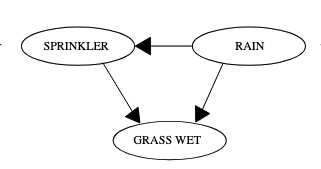
\includegraphics[width=.6\textwidth]{figures/image1.png}\\
    Source: Wikipedia 
\end{center}
\noindent We can then define prior and conditional probabilities to "back out" the probability of rain. In order to cover every scenario, we require prior probabilities for all the nodes with no edges entering them, and posterior probabilities for all the edges relating multiple nodes. Suppose $\PrMe(R) = 0.2$, $\PrMe(S|R) = 0.1$, $\PrMe(S|\sim R) = 0.6$, $\PrMe(G|R, S) = 1$, $\PrMe(G|R, \sim S) = 0.8$, $\PrMe(G | \sim R, S) = 0.9$, and $\PrMe(G|\sim R, \sim S) = 0$. We seek $\PrMe(R|G)$, the probability it rained given that we observe wet grass. From Bayes' rule we have
$$\PrMe(R|G) = \frac{\PrMe(G \cap R)}{\PrMe(G)} = \frac{\sum_{s \in S}\PrMe(G, R, S=s)}{\sum_{s \in S, r \in R}\PrMe(G, R=r, S=s)}$$
The numerator is the probability that it rained and that the grass is wet, regardless of whether the sprinkler operated. We can then substitute
\begin{align*}
\sum_{s \in S}\PrMe(G, R, S=s) &= \PrMe(G, R, S) + \PrMe(G, R, \sim S) \\
&= \PrMe(G | R, S)\PrMe(S | R)\PrMe(R) + \PrMe(G|R, \sim S)\PrMe(\sim S | R)\PrMe(R) \\
&= 1(0.1)(0.2) + 0.8(0.9)(0.2) = 0.164
\end{align*}
The denominator is the probability that the grass is wet, regardless of whether it rained or not. We know that the probability the grass is wet given it did rain is 0.164, so we just need to calculate the probability given that it didn't. This is given by
\begin{align*}
\sum_{s \in S}\PrMe(G, \sim R, S=s) &= \PrMe(G, \sim R, S) + \PrMe(G, \sim R, \sim S) \\
&= \PrMe(G | \sim R, S)\PrMe(S | \sim R)\PrMe(\sim R) + \PrMe(G| \sim R, \sim S)\PrMe(\sim S | \sim R)\PrMe(\sim R) \\
&= 0.9(0.6)(0.8) + 0 = 0.432
\end{align*}
Therefore, $\PrMe (R | G) = \frac{0.164}{0.164 + 0.432} \approx 0.275$. \\\\
While Bayes nets may be relatively simple, they are a key first step to understanding other models which extend this logic to more complex systems with some observable random variables and other hidden state variables, such as hidden Markov models and Kalman filters. These models continuously update their probability distributions based on observations from data, and are useful in situations in which the true probability distribution is not known. They and others like them may be encountered in CS 188, CS 189, or other upper-division or graduate courses involving probabilistic modeling.

\end{document}